

\chapter{Preliminaries}
\label{ch:preliminaries}

In this chapter, we intend to provide a background for the terms and the dataset we use in the thesis. We will refer back to this chapter when needed in the text. 

\section{Distance Metrics}

In our solutions presented we order the database of items based on their similarity/distance to the query. We use cosine distance and euclidean distance. We experiment with those metrics, based on the disadvantages of the euclidean distance in higher dimensionality spaces.

\subsection{Cosine Distance}

We use following version of cosine distance based on the cosine similarity.

\begin{equation}
\text{similarity} = \cos ({\bf p},{\bf q})= {{\bf p} {\bf q} \over \|{\bf p}\| \|{\bf q}\|} = \frac{ \sum_{i=1}^{n}{{\bf p}_i{\bf q}_i} }{ \sqrt{\sum_{i=1}^{n}{{\bf p}_i^2}} \sqrt{\sum_{i=1}^{n}{{\bf q}_i^2}} }
\end{equation}

\begin{equation}
    \text{cos\_distance} = 1 - \text{similarity}
\end{equation}

\subsection{Euclidean Distance}
\begin{equation}
d(p, q) = \sqrt{\sum_{i=1}^n (p_i - q_i)^2}    
\end{equation}

\section{Dataset}
\label{s:dataset}

We use Vimeo Creative Commons Collections (V3C1)\footnote{\href{https://www-nlpir.nist.gov/projects/tv2019/data.html}{TRECVID 2019 Video Data}} dataset for experimenting and evaluations. The dataset is composed of 7475 Vimeo videos. We selected only the first 750 videos for proving concepts of our work. From these 750 videos, we used an extraction tool from VIRET \cite{lokovc2019framework}. After extraction, we obtained 111\ 764 images from 750 videos with resolution 320x180.

The videos capture a wide range of sceneries on many different occasions. We can see many different landscapes, from seas to mountain views, from desert to snow. A large proportion of the videos contain people. Videos capture people doing different activities, i.e., from Hindi wedding to skateboarding in a park or a news broadcast.

\subsection{Collages used for evaluation}

In the chapter \ref{ch:object_location} we do different evaluations of proposed systems. To do that in a known-search item task, we beforehand annotated a set of the data. The data consist of 100 collages, all containing a visual image description of a given scene. The average size of the images used in the collages covers 15\% of the canvas. Five \% of the dataset consists of images bigger than 80\% of the canvas. We provide visualization of the distribution of the annotated queries in figure \ref{fig:annotated_dataset}.

For the annotation, we used our application used for spatial queries. It is possible to save the collage by clicking "Submit Collage." The average time spends on annotation one image was 91 seconds. This time includes searching for images online, pasting them onto the canvas, and usually also waiting for the query to go through. The majority of the time is spent by looking for a good match in the image search engine.

\begin{figure}
     \centering
     \begin{subfigure}[b]{0.48\textwidth}
         \centering
         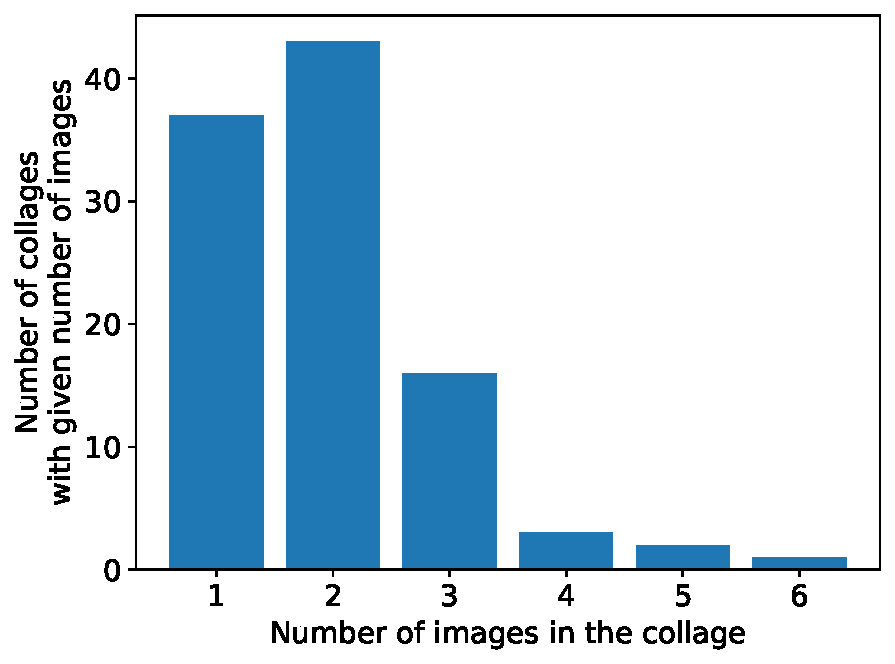
\includegraphics[width=\textwidth]{graphs/num_queries_in_request.pdf}
         \caption{Number of images on a canvas for a collage.}
         \label{fig:y equals x}
     \end{subfigure}
     \hfill
     \begin{subfigure}[b]{0.48\textwidth}
         \centering
         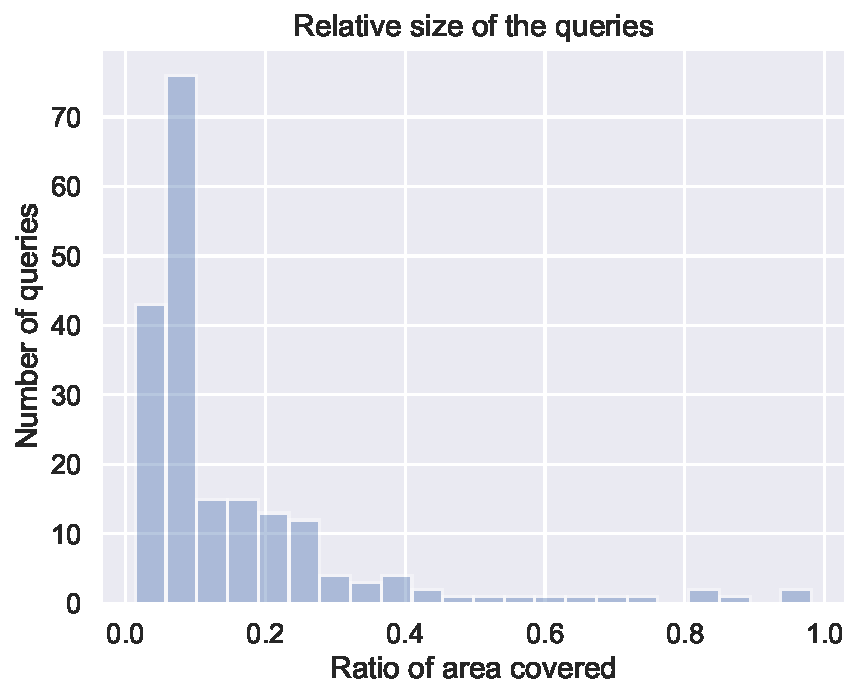
\includegraphics[width=\textwidth]{graphs/queries_size.pdf}
         \caption{Size of the canvas which is covered by a query image.}
         \label{fig:three sin x}
     \end{subfigure}
    
    \caption{Annotated collages properties}
    \label{fig:annotated_dataset}
\end{figure}


\section{Intersection over Union}

In the following chapters, we use Intersection over Union (IoU) as a characteristic of overlapping. Intersection over Union (also known as Jaccard index\footnote{\href{https://en.wikipedia.org/wiki/Jaccard_index}{https://en.wikipedia.org/wiki/Jaccard\_index}}) measures similarity between two sets. We use it as a metric to express how much two regions (i.e., two rectangles) overlap. 

The definitions of the Interectio over Union is as follows:
$$
    J(A, B) = 
    \begin{cases}
      1, & \text{if\ A and B are empty} \\
      \frac{|A \cap B|}{|A \cup B|}, & \text{otherwise}
    \end{cases}
$$

In our case, the $|A \cap B|$ represents the are belonging to both regions. The  $|A \cup B|$ represents the area covered by union of the both regions. A visual representation of the fomrula is displayed in the Figure \ref{fig:intersection_over_union}.

\begin{figure}
    \centering
	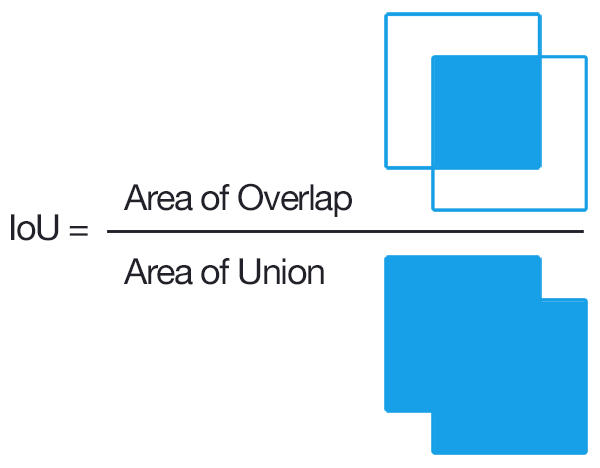
\includegraphics[width=0.3\linewidth]{img/Intersection_over_Union_-_visual_equation.png}
	\caption{Intersection over Union between regions. Source: Wikipedia, CC BY-SA 4.0}
	\label{fig:intersection_over_union}
\end{figure}




% We consider a known set of images I and a query Q∈ I. We utilize a representation ^Q over Q, such that minimize search_rank(^Q, I). We define search_rank as an ordering function based on similarity function (or inverse of distance function). We focus on testing different representations ^Q for query Q.  




